\documentclass[t, aspectratio=169]{beamer}
\usepackage{amsmath,amsfonts,amsthm,amstext,amssymb, xcolor, tikz, pgf, mathrsfs, polynom, pifont, tabto}

% ----------------------------------------------------------
% Theme Setup

% Use Metropolis Theme
\usetheme[numbering=fraction]{metropolis}
\setbeamertemplate{blocks}[rounded][shadow=false]
\makeatletter
\setlength{\metropolis@titleseparator@linewidth}{1pt}
\makeatother

% Define Colors
\definecolor{chargerblue}{HTML}{002764}
\definecolor{chargerred}{HTML}{e02034}
\definecolor{bggray}{HTML}{d0d3d4}

% Set Colors
\setbeamercolor{title}{fg=chargerblue}
\setbeamercolor{background canvas}{bg=white}
\setbeamercolor{title separator}{fg=chargerred}
\setbeamercolor{structure}{fg=chargerblue}
\setbeamercolor{frametitle}{fg=white, bg=chargerblue}
\setbeamercolor*{normal text}{fg=chargerblue}
\setbeamercolor*{block body}{bg=bggray}
\setbeamercolor*{block title}{bg=chargerblue, fg=white}
% ----------------------------------------------------------

% ----------------------------------------------------------
% Custom Definitions, Commands, Environments, etc.

% Sets of numbers
\def\R{\mathbb{R}} % The reals
\def\N{\mathbb{N}} % The naturals
\def\Z{\mathbb{Z}} % The integers
\def\Q{\mathbb{Q}} % The rationals

% Blank space
\newcommand{\blank}[1]{\underline{\hspace{#1}}} % Blank space

% Change font colors
\newcommand{\cyan}[1]{{\color{cyan}{#1}}} % Changes font to cyan
\newcommand{\red}[1]{{\color{red}{#1}}} % Changes font to red
\newcommand{\magenta}[1]{{\color{magenta}{#1}}} % Changes font to magenta
\newcommand{\orange}[1]{{\color{orange}{#1}}} % Changes font to orange
\newcommand{\yellow}[1]{{\color{yellow}{#1}}} % Changes font to yellow
\newcommand{\violet}[1]{{\color{violet}{#1}}} % Changes font to violet
\newcommand{\green}[1]{{\color{green}{#1}}} % Changes font to green
\newcommand{\blue}[1]{{\color{blue}{#1}}} % Changes font to blue
\newcommand{\white}[1]{{\color{white}{#1}}} % Changes font to white

% Fitted inclusion symbols
\newcommand{\fp}[1]{\left({#1}\right)} % Fitted parentheses around content
\newcommand{\fb}[1]{\left[{#1}\right]} % Fitted brackets
\newcommand{\lhoi}[1]{\left({#1}\right]} % Left half-open interval
\newcommand{\rhoi}[1]{\left[{#1}\right)} % Right half-open interval
\newcommand{\set}[1]{\left\{{#1}\right\}} % Fitted braces (useful for sets)
\newcommand{\av}[1]{\left|{#1}\right|} % Fitted absolute value bars

% Augmented Matrix Environment
\newenvironment{amatrix}[1]{%
	\left[\begin{array}{@{}*{#1}{c}|c@{}}
	}{%
	\end{array}\right]
}

% Miscellaneous
\def\then{\Rightarrow}
\def\to{\rightarrow}
\def\d{^{\circ}}
\newcommand{\?}{\stackrel{?}{=}}
\newcommand{\cmark}{\text{ \ding{51}}}
\newcommand{\xmark}{\text{ \ding{55}}}

% Coordinate Plane (Four-Quadrant)
\def\coordplane {
	\begin{tikzpicture}        \draw[step=0.25cm,black,very thin,opacity=0.25] (-2.5cm, -2.5cm) grid (2.5cm, 2.5cm);
	\draw[<->,thick,black] (-2.5cm, 0) -- (2.5cm, 0) node[anchor=north west,pos=0.94,font=\scriptsize]{$x$};
	\draw[<->,thick,black] (0,-2.5cm) -- (0, 2.5cm) node[anchor=south east,font=\scriptsize,pos=0.94]{$y$};
	\end{tikzpicture}
}

% Coordinate Plane (One-Quadrant)
\def\onequad {
	\begin{tikzpicture}
	\draw[step=0.25cm, black, very thin, opacity=0.25] (0,0) grid (7.5cm,5cm);
	\draw[->, thick, black] (0,0) -- (7.5cm, 0) node[anchor=north west,font=\scriptsize,pos=0.94]{$x$};
	\draw[->, black, thick] (0,0) -- (0,5cm) node[anchor=south east,font=\scriptsize,pos=0.94]{$y$};
	\end{tikzpicture}
}
% ----------------------------------------------------------

% ----------------------------------------------------------
% Presentation Information
\title[8-1]{Steps to Hypothesis Testing}
\subtitle{Section 8-1}
\author{Jacob Ayers}
\institute{Lesson \#24}
\date{MAT 110}
% ----------------------------------------------------------

\begin{document}
	
	% Slide 1 (Title Slide)
	\begin{frame}
		\titlepage
	\end{frame}
	
	% Slide 2 (Objectives)
	\begin{frame}{Objectives}
		\begin{itemize}
			\item Understand the definitions used in hypothesis testing
			\item State the null and alternative hypotheses
			\item Identify type I error and type II error
			\item Find critical values for the $z$ test
		\end{itemize}
	\end{frame}

	\begin{frame}{Key Definitions}
		A \textit{statistical hypothesis} is a conjecture about a population parameter; it may or may not be true. \pause
		
		When performing hypothesis tests, there are always two hypotheses: \pause
		
		Null hypothesis ($H_0$): states that there is no difference between a parameter and a specific value. \begin{itemize}
			\item Includes an $=$ sign
		\end{itemize} \pause
		
		Alternative hypothesis ($H_1$): states that there is a difference between a parameter and a specific value. \begin{itemize}
			\item Includes either $>$, $<$, or $\neq$
		\end{itemize} \pause
	\end{frame}

	\begin{frame}{Null and Alternative Hypotheses}
		\textbf{Situation A} A medical researcher is interested in finding out whether a new medication will have any undesirable side effects. The researcher is particularly concerned with the pulse rate of patients who take the medication. Will the pulse rate increase, decrease, or remain unchanged after a patient takes the medication?
		The researcher knows the mean pulse rate for the population under study is 82 beats per minute. \pause
		
		The null hypothesis states that there is no difference. \pause
		
		So the null hypothesis is: $H_0: \; \mu = 82$ \pause
		
		In this case, we are interested in \textit{change}. There is change if the heart rate increases or decreases. \pause
		
		So the alternative hypothesis is: $H_1: \; \mu \neq 82$ \pause
		
		This is an example of a \textit{two-tailed test}.
	\end{frame}

	\begin{frame}{Null and Alternative Hypotheses}
		\textbf{Situation B} A chemist invents an additive to increase the life of an automobile battery. The mean lifetime of the battery without the additive is 36 months. \pause
		
		$H_0: \; \mu = 36$ \pause
		
		This time, we're only interested in an \textit{increase}. \pause
		
		So the alternative hypothesis is: $H_1: \; \mu > 36$ \pause
		
		This is an example of a \textit{right-tailed test}.
	\end{frame}

	\begin{frame}{Null and Alternative Hypotheses}
		\textbf{Situation C} A contractor wishes to lower heating bills by using a special type of insulation in houses. The average monthly heating bill is \$78. \pause
		
		$H_0: \; \mu = 78$ \pause
		
		This time, we're only interested in a \textit{decrease}. \pause
		
		So the alternative hypothesis is: $H_1: \; \mu < 78$ \pause
		
		This is an example of a \textit{left-tailed test}. \pause
		
		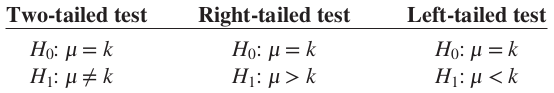
\includegraphics[width=4in]{test-summary.png}
	\end{frame}

	\begin{frame}{Null and Alternative Hypotheses}
		State the null and alternative hypotheses for each situation: \begin{enumerate}[a)]
			\item A researcher studies gambling in young people. She thinks those who gamble spend more than \$30 per day.
			\item A researcher wishes to see if police officers who work in law enforcement have a lower score on a work stress test questionnaire than the average score of 120.
			\item A teacher feels that if an online textbook is used for a course instead of a hardback book, it may change the students' scores on the final exam. In the past, the average final exam score for the students was 83.
		\end{enumerate} \pause
	
		a) $H_0: \mu = 30$ and $H_1: \mu > 30$ \pause \\
		b) $H_0: \mu = 120$ and $H_1: \mu < 120$ \pause \\
		c) $H_0: \mu = 83$ and $H_1: \mu \neq 83$
	\end{frame}

	\begin{frame}{Statistical Tests}
		Stating the null and alternative hypotheses is the first step in hypothesis testing. \pause
		
		The next step is identifying the correct statistical test to use. \pause
		
		A \textit{statistical test} uses the data obtained from a sample to make a decision about whether the null hypothesis should be rejected. \pause
		
		The numerical value obtained from a statistical test is called the \textit{test value} or \textit{test statistic}.
	\end{frame}

	\begin{frame}{Errors in Decision-Making}
		There are four possible outcomes in a hypothesis test: \pause \begin{enumerate}[1)]
			\item Reject $H_0$ when $H_0$ is true (Type I Error) \pause
			\item Reject $H_0$ when $H_0$ is false (Correct Decision) \pause
			\item Do not reject $H_0$ when $H_0$ is true (Correct Decision) \pause
			\item Do not reject $H_0$ when $H_0$ is false (Type II Error) \pause
		\end{enumerate}
	
		To clarify, let's look at this in context of a trial. \pause
		
		Either the defendant is innocent or guilty, and the jury either convicts or acquits the defendant.
	\end{frame}

	\begin{frame}{Errors in Decision-Making}
		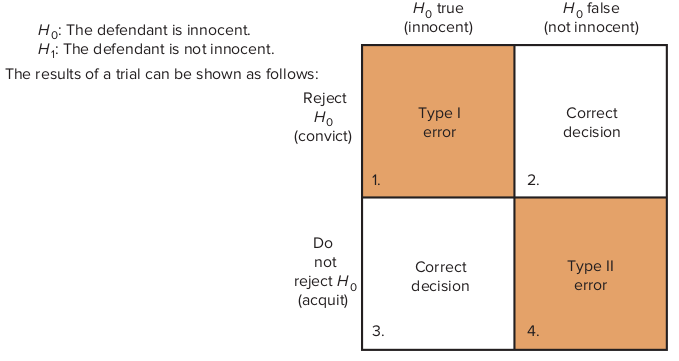
\includegraphics[width=0.85\textwidth]{error-example.png}
	\end{frame}

	\begin{frame}{Level of Significance}
		Key point: Jury's decision does not prove that the defendant did or did not commit the crime. \pause
		
		There is a possibility that a type I error or type II error occurred. \pause
		
		The only way to prove anything statistically is to use the entire population - this is almost always impossible. \pause
		
		So how do we make decisions? \pause We use probability. \pause
		
		If there is a big difference between the mean of a sample mean and the hypothesized mean, the hypothesized mean is probably wrong. \pause
		
		So how big is "big"? \pause
		
		We use the \textit{level of significance} to answer this question.
	\end{frame}

	\begin{frame}{Level of Significance}
		The \textit{level of significance} ($\alpha$) is the maximum probability of committing a type I error. \pause
		
		Statisticians usually use either $\alpha = 0.10$, $\alpha = 0.05$, or $\alpha = 0.01$ as the significance level. \pause
		
		The significance level depends on how serious a type I error is. \pause
		
		Once a significance level is chosen, a critical value is found using a table from an appropriate test. \pause
		
		This critical value is used to determine the critical and noncritical regions.
	\end{frame}
	
	\begin{frame}{Critical and Noncritical Regions}
		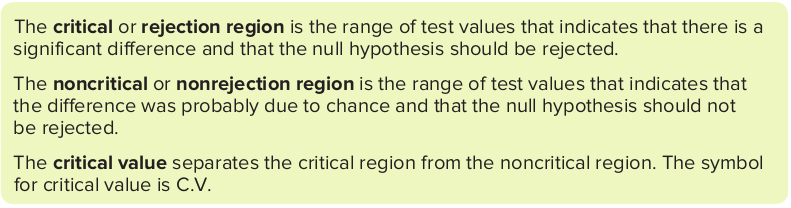
\includegraphics[width=\textwidth]{regions.png} \pause
		
		If the test is a one-tailed test, then the size of the critical region is equal to the alpha level. \pause
		
		If the test is a two-tailed test, then there are two critical regions, each with an area of half the alpha level. \pause
		
		Drawing a picture to represent the situation is very useful.
	\end{frame}

	\begin{frame}{Critical and Noncritical Regions}
		Draw the critical and noncritical regions for a two-tailed test with $\alpha = 0.05$.
	\end{frame}

	\begin{frame}{Critical and Noncritical Regions}
		Draw the critical and noncritical regions for a left-tailed test with $\alpha = 0.10$.
	\end{frame}

	\begin{frame}{Critical and Noncritical Regions}
		Draw the critical and noncritical regions for a right-tailed test with $\alpha = 0.01$.
	\end{frame}

	\begin{frame}{Finding Critical Values with the $z$ Table}
		Draw the appropriate figure and find the critical value for a right-tailed test with $\alpha = 0.05$ using the $z$ table.
	\end{frame}

	\begin{frame}{Finding Critical Values with the $z$ Table}
		Draw the appropriate figure and find the critical value for a two-tailed test with $\alpha = 0.02$ using the $z$ table.
	\end{frame}

	\begin{frame}{Finding Critical Values with the $z$ Table}
		Draw the appropriate figure and find the critical value for a left-tailed test with $\alpha = 0.03$ using the $z$ table.
	\end{frame}

	\begin{frame}{Hypothesis Testing Process}
		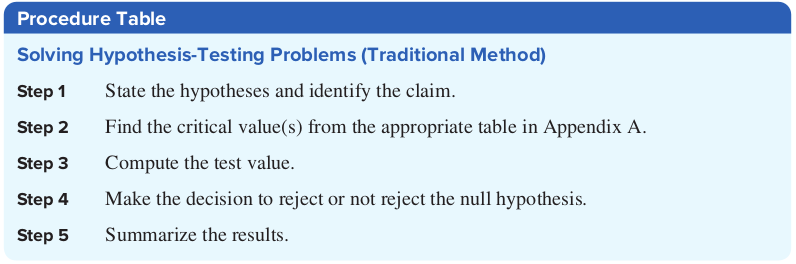
\includegraphics[width=\textwidth]{hyp-process.png} \pause
		
		We focused on Steps 1 and 2 of this process here. In the next lesson, we'll solve hypothesis-testing problems using the $z$ test for the mean.
	\end{frame}

	\begin{frame}{Next Steps}
		\begin{itemize}
			\item Read 8-2
			\item Watch Video Lesson \#25
			\item Complete Assignment 12
		\end{itemize}
	
		\vfill
		
		Thanks for watching!
	\end{frame}
\end{document}